\documentclass{article} % For LaTeX2e
\usepackage{iclr2025_conference,times}
%%%%% NEW MATH DEFINITIONS %%%%%

\usepackage{amsmath,amsfonts,bm}

% Mark sections of captions for referring to divisions of figures
\newcommand{\figleft}{{\em (Left)}}
\newcommand{\figcenter}{{\em (Center)}}
\newcommand{\figright}{{\em (Right)}}
\newcommand{\figtop}{{\em (Top)}}
\newcommand{\figbottom}{{\em (Bottom)}}
\newcommand{\captiona}{{\em (a)}}
\newcommand{\captionb}{{\em (b)}}
\newcommand{\captionc}{{\em (c)}}
\newcommand{\captiond}{{\em (d)}}

% Highlight a newly defined term
\newcommand{\newterm}[1]{{\bf #1}}


% Figure reference, lower-case.
\def\figref#1{figure~\ref{#1}}
% Figure reference, capital. For start of sentence
\def\Figref#1{Figure~\ref{#1}}
\def\twofigref#1#2{figures \ref{#1} and \ref{#2}}
\def\quadfigref#1#2#3#4{figures \ref{#1}, \ref{#2}, \ref{#3} and \ref{#4}}
% Section reference, lower-case.
\def\secref#1{section~\ref{#1}}
% Section reference, capital.
\def\Secref#1{Section~\ref{#1}}
% Reference to two sections.
\def\twosecrefs#1#2{sections \ref{#1} and \ref{#2}}
% Reference to three sections.
\def\secrefs#1#2#3{sections \ref{#1}, \ref{#2} and \ref{#3}}
% Reference to an equation, lower-case.
\def\eqref#1{equation~\ref{#1}}
% Reference to an equation, upper case
\def\Eqref#1{Equation~\ref{#1}}
% A raw reference to an equation---avoid using if possible
\def\plaineqref#1{\ref{#1}}
% Reference to a chapter, lower-case.
\def\chapref#1{chapter~\ref{#1}}
% Reference to an equation, upper case.
\def\Chapref#1{Chapter~\ref{#1}}
% Reference to a range of chapters
\def\rangechapref#1#2{chapters\ref{#1}--\ref{#2}}
% Reference to an algorithm, lower-case.
\def\algref#1{algorithm~\ref{#1}}
% Reference to an algorithm, upper case.
\def\Algref#1{Algorithm~\ref{#1}}
\def\twoalgref#1#2{algorithms \ref{#1} and \ref{#2}}
\def\Twoalgref#1#2{Algorithms \ref{#1} and \ref{#2}}
% Reference to a part, lower case
\def\partref#1{part~\ref{#1}}
% Reference to a part, upper case
\def\Partref#1{Part~\ref{#1}}
\def\twopartref#1#2{parts \ref{#1} and \ref{#2}}

\def\ceil#1{\lceil #1 \rceil}
\def\floor#1{\lfloor #1 \rfloor}
\def\1{\bm{1}}
\newcommand{\train}{\mathcal{D}}
\newcommand{\valid}{\mathcal{D_{\mathrm{valid}}}}
\newcommand{\test}{\mathcal{D_{\mathrm{test}}}}

\def\eps{{\epsilon}}


% Random variables
\def\reta{{\textnormal{$\eta$}}}
\def\ra{{\textnormal{a}}}
\def\rb{{\textnormal{b}}}
\def\rc{{\textnormal{c}}}
\def\rd{{\textnormal{d}}}
\def\re{{\textnormal{e}}}
\def\rf{{\textnormal{f}}}
\def\rg{{\textnormal{g}}}
\def\rh{{\textnormal{h}}}
\def\ri{{\textnormal{i}}}
\def\rj{{\textnormal{j}}}
\def\rk{{\textnormal{k}}}
\def\rl{{\textnormal{l}}}
% rm is already a command, just don't name any random variables m
\def\rn{{\textnormal{n}}}
\def\ro{{\textnormal{o}}}
\def\rp{{\textnormal{p}}}
\def\rq{{\textnormal{q}}}
\def\rr{{\textnormal{r}}}
\def\rs{{\textnormal{s}}}
\def\rt{{\textnormal{t}}}
\def\ru{{\textnormal{u}}}
\def\rv{{\textnormal{v}}}
\def\rw{{\textnormal{w}}}
\def\rx{{\textnormal{x}}}
\def\ry{{\textnormal{y}}}
\def\rz{{\textnormal{z}}}

% Random vectors
\def\rvepsilon{{\mathbf{\epsilon}}}
\def\rvtheta{{\mathbf{\theta}}}
\def\rva{{\mathbf{a}}}
\def\rvb{{\mathbf{b}}}
\def\rvc{{\mathbf{c}}}
\def\rvd{{\mathbf{d}}}
\def\rve{{\mathbf{e}}}
\def\rvf{{\mathbf{f}}}
\def\rvg{{\mathbf{g}}}
\def\rvh{{\mathbf{h}}}
\def\rvu{{\mathbf{i}}}
\def\rvj{{\mathbf{j}}}
\def\rvk{{\mathbf{k}}}
\def\rvl{{\mathbf{l}}}
\def\rvm{{\mathbf{m}}}
\def\rvn{{\mathbf{n}}}
\def\rvo{{\mathbf{o}}}
\def\rvp{{\mathbf{p}}}
\def\rvq{{\mathbf{q}}}
\def\rvr{{\mathbf{r}}}
\def\rvs{{\mathbf{s}}}
\def\rvt{{\mathbf{t}}}
\def\rvu{{\mathbf{u}}}
\def\rvv{{\mathbf{v}}}
\def\rvw{{\mathbf{w}}}
\def\rvx{{\mathbf{x}}}
\def\rvy{{\mathbf{y}}}
\def\rvz{{\mathbf{z}}}

% Elements of random vectors
\def\erva{{\textnormal{a}}}
\def\ervb{{\textnormal{b}}}
\def\ervc{{\textnormal{c}}}
\def\ervd{{\textnormal{d}}}
\def\erve{{\textnormal{e}}}
\def\ervf{{\textnormal{f}}}
\def\ervg{{\textnormal{g}}}
\def\ervh{{\textnormal{h}}}
\def\ervi{{\textnormal{i}}}
\def\ervj{{\textnormal{j}}}
\def\ervk{{\textnormal{k}}}
\def\ervl{{\textnormal{l}}}
\def\ervm{{\textnormal{m}}}
\def\ervn{{\textnormal{n}}}
\def\ervo{{\textnormal{o}}}
\def\ervp{{\textnormal{p}}}
\def\ervq{{\textnormal{q}}}
\def\ervr{{\textnormal{r}}}
\def\ervs{{\textnormal{s}}}
\def\ervt{{\textnormal{t}}}
\def\ervu{{\textnormal{u}}}
\def\ervv{{\textnormal{v}}}
\def\ervw{{\textnormal{w}}}
\def\ervx{{\textnormal{x}}}
\def\ervy{{\textnormal{y}}}
\def\ervz{{\textnormal{z}}}

% Random matrices
\def\rmA{{\mathbf{A}}}
\def\rmB{{\mathbf{B}}}
\def\rmC{{\mathbf{C}}}
\def\rmD{{\mathbf{D}}}
\def\rmE{{\mathbf{E}}}
\def\rmF{{\mathbf{F}}}
\def\rmG{{\mathbf{G}}}
\def\rmH{{\mathbf{H}}}
\def\rmI{{\mathbf{I}}}
\def\rmJ{{\mathbf{J}}}
\def\rmK{{\mathbf{K}}}
\def\rmL{{\mathbf{L}}}
\def\rmM{{\mathbf{M}}}
\def\rmN{{\mathbf{N}}}
\def\rmO{{\mathbf{O}}}
\def\rmP{{\mathbf{P}}}
\def\rmQ{{\mathbf{Q}}}
\def\rmR{{\mathbf{R}}}
\def\rmS{{\mathbf{S}}}
\def\rmT{{\mathbf{T}}}
\def\rmU{{\mathbf{U}}}
\def\rmV{{\mathbf{V}}}
\def\rmW{{\mathbf{W}}}
\def\rmX{{\mathbf{X}}}
\def\rmY{{\mathbf{Y}}}
\def\rmZ{{\mathbf{Z}}}

% Elements of random matrices
\def\ermA{{\textnormal{A}}}
\def\ermB{{\textnormal{B}}}
\def\ermC{{\textnormal{C}}}
\def\ermD{{\textnormal{D}}}
\def\ermE{{\textnormal{E}}}
\def\ermF{{\textnormal{F}}}
\def\ermG{{\textnormal{G}}}
\def\ermH{{\textnormal{H}}}
\def\ermI{{\textnormal{I}}}
\def\ermJ{{\textnormal{J}}}
\def\ermK{{\textnormal{K}}}
\def\ermL{{\textnormal{L}}}
\def\ermM{{\textnormal{M}}}
\def\ermN{{\textnormal{N}}}
\def\ermO{{\textnormal{O}}}
\def\ermP{{\textnormal{P}}}
\def\ermQ{{\textnormal{Q}}}
\def\ermR{{\textnormal{R}}}
\def\ermS{{\textnormal{S}}}
\def\ermT{{\textnormal{T}}}
\def\ermU{{\textnormal{U}}}
\def\ermV{{\textnormal{V}}}
\def\ermW{{\textnormal{W}}}
\def\ermX{{\textnormal{X}}}
\def\ermY{{\textnormal{Y}}}
\def\ermZ{{\textnormal{Z}}}

% Vectors
\def\vzero{{\bm{0}}}
\def\vone{{\bm{1}}}
\def\vmu{{\bm{\mu}}}
\def\vtheta{{\bm{\theta}}}
\def\va{{\bm{a}}}
\def\vb{{\bm{b}}}
\def\vc{{\bm{c}}}
\def\vd{{\bm{d}}}
\def\ve{{\bm{e}}}
\def\vf{{\bm{f}}}
\def\vg{{\bm{g}}}
\def\vh{{\bm{h}}}
\def\vi{{\bm{i}}}
\def\vj{{\bm{j}}}
\def\vk{{\bm{k}}}
\def\vl{{\bm{l}}}
\def\vm{{\bm{m}}}
\def\vn{{\bm{n}}}
\def\vo{{\bm{o}}}
\def\vp{{\bm{p}}}
\def\vq{{\bm{q}}}
\def\vr{{\bm{r}}}
\def\vs{{\bm{s}}}
\def\vt{{\bm{t}}}
\def\vu{{\bm{u}}}
\def\vv{{\bm{v}}}
\def\vw{{\bm{w}}}
\def\vx{{\bm{x}}}
\def\vy{{\bm{y}}}
\def\vz{{\bm{z}}}

% Elements of vectors
\def\evalpha{{\alpha}}
\def\evbeta{{\beta}}
\def\evepsilon{{\epsilon}}
\def\evlambda{{\lambda}}
\def\evomega{{\omega}}
\def\evmu{{\mu}}
\def\evpsi{{\psi}}
\def\evsigma{{\sigma}}
\def\evtheta{{\theta}}
\def\eva{{a}}
\def\evb{{b}}
\def\evc{{c}}
\def\evd{{d}}
\def\eve{{e}}
\def\evf{{f}}
\def\evg{{g}}
\def\evh{{h}}
\def\evi{{i}}
\def\evj{{j}}
\def\evk{{k}}
\def\evl{{l}}
\def\evm{{m}}
\def\evn{{n}}
\def\evo{{o}}
\def\evp{{p}}
\def\evq{{q}}
\def\evr{{r}}
\def\evs{{s}}
\def\evt{{t}}
\def\evu{{u}}
\def\evv{{v}}
\def\evw{{w}}
\def\evx{{x}}
\def\evy{{y}}
\def\evz{{z}}

% Matrix
\def\mA{{\bm{A}}}
\def\mB{{\bm{B}}}
\def\mC{{\bm{C}}}
\def\mD{{\bm{D}}}
\def\mE{{\bm{E}}}
\def\mF{{\bm{F}}}
\def\mG{{\bm{G}}}
\def\mH{{\bm{H}}}
\def\mI{{\bm{I}}}
\def\mJ{{\bm{J}}}
\def\mK{{\bm{K}}}
\def\mL{{\bm{L}}}
\def\mM{{\bm{M}}}
\def\mN{{\bm{N}}}
\def\mO{{\bm{O}}}
\def\mP{{\bm{P}}}
\def\mQ{{\bm{Q}}}
\def\mR{{\bm{R}}}
\def\mS{{\bm{S}}}
\def\mT{{\bm{T}}}
\def\mU{{\bm{U}}}
\def\mV{{\bm{V}}}
\def\mW{{\bm{W}}}
\def\mX{{\bm{X}}}
\def\mY{{\bm{Y}}}
\def\mZ{{\bm{Z}}}
\def\mBeta{{\bm{\beta}}}
\def\mPhi{{\bm{\Phi}}}
\def\mLambda{{\bm{\Lambda}}}
\def\mSigma{{\bm{\Sigma}}}

% Tensor
\DeclareMathAlphabet{\mathsfit}{\encodingdefault}{\sfdefault}{m}{sl}
\SetMathAlphabet{\mathsfit}{bold}{\encodingdefault}{\sfdefault}{bx}{n}
\newcommand{\tens}[1]{\bm{\mathsfit{#1}}}
\def\tA{{\tens{A}}}
\def\tB{{\tens{B}}}
\def\tC{{\tens{C}}}
\def\tD{{\tens{D}}}
\def\tE{{\tens{E}}}
\def\tF{{\tens{F}}}
\def\tG{{\tens{G}}}
\def\tH{{\tens{H}}}
\def\tI{{\tens{I}}}
\def\tJ{{\tens{J}}}
\def\tK{{\tens{K}}}
\def\tL{{\tens{L}}}
\def\tM{{\tens{M}}}
\def\tN{{\tens{N}}}
\def\tO{{\tens{O}}}
\def\tP{{\tens{P}}}
\def\tQ{{\tens{Q}}}
\def\tR{{\tens{R}}}
\def\tS{{\tens{S}}}
\def\tT{{\tens{T}}}
\def\tU{{\tens{U}}}
\def\tV{{\tens{V}}}
\def\tW{{\tens{W}}}
\def\tX{{\tens{X}}}
\def\tY{{\tens{Y}}}
\def\tZ{{\tens{Z}}}


% Graph
\def\gA{{\mathcal{A}}}
\def\gB{{\mathcal{B}}}
\def\gC{{\mathcal{C}}}
\def\gD{{\mathcal{D}}}
\def\gE{{\mathcal{E}}}
\def\gF{{\mathcal{F}}}
\def\gG{{\mathcal{G}}}
\def\gH{{\mathcal{H}}}
\def\gI{{\mathcal{I}}}
\def\gJ{{\mathcal{J}}}
\def\gK{{\mathcal{K}}}
\def\gL{{\mathcal{L}}}
\def\gM{{\mathcal{M}}}
\def\gN{{\mathcal{N}}}
\def\gO{{\mathcal{O}}}
\def\gP{{\mathcal{P}}}
\def\gQ{{\mathcal{Q}}}
\def\gR{{\mathcal{R}}}
\def\gS{{\mathcal{S}}}
\def\gT{{\mathcal{T}}}
\def\gU{{\mathcal{U}}}
\def\gV{{\mathcal{V}}}
\def\gW{{\mathcal{W}}}
\def\gX{{\mathcal{X}}}
\def\gY{{\mathcal{Y}}}
\def\gZ{{\mathcal{Z}}}

% Sets
\def\sA{{\mathbb{A}}}
\def\sB{{\mathbb{B}}}
\def\sC{{\mathbb{C}}}
\def\sD{{\mathbb{D}}}
% Don't use a set called E, because this would be the same as our symbol
% for expectation.
\def\sF{{\mathbb{F}}}
\def\sG{{\mathbb{G}}}
\def\sH{{\mathbb{H}}}
\def\sI{{\mathbb{I}}}
\def\sJ{{\mathbb{J}}}
\def\sK{{\mathbb{K}}}
\def\sL{{\mathbb{L}}}
\def\sM{{\mathbb{M}}}
\def\sN{{\mathbb{N}}}
\def\sO{{\mathbb{O}}}
\def\sP{{\mathbb{P}}}
\def\sQ{{\mathbb{Q}}}
\def\sR{{\mathbb{R}}}
\def\sS{{\mathbb{S}}}
\def\sT{{\mathbb{T}}}
\def\sU{{\mathbb{U}}}
\def\sV{{\mathbb{V}}}
\def\sW{{\mathbb{W}}}
\def\sX{{\mathbb{X}}}
\def\sY{{\mathbb{Y}}}
\def\sZ{{\mathbb{Z}}}

% Entries of a matrix
\def\emLambda{{\Lambda}}
\def\emA{{A}}
\def\emB{{B}}
\def\emC{{C}}
\def\emD{{D}}
\def\emE{{E}}
\def\emF{{F}}
\def\emG{{G}}
\def\emH{{H}}
\def\emI{{I}}
\def\emJ{{J}}
\def\emK{{K}}
\def\emL{{L}}
\def\emM{{M}}
\def\emN{{N}}
\def\emO{{O}}
\def\emP{{P}}
\def\emQ{{Q}}
\def\emR{{R}}
\def\emS{{S}}
\def\emT{{T}}
\def\emU{{U}}
\def\emV{{V}}
\def\emW{{W}}
\def\emX{{X}}
\def\emY{{Y}}
\def\emZ{{Z}}
\def\emSigma{{\Sigma}}

% entries of a tensor
% Same font as tensor, without \bm wrapper
\newcommand{\etens}[1]{\mathsfit{#1}}
\def\etLambda{{\etens{\Lambda}}}
\def\etA{{\etens{A}}}
\def\etB{{\etens{B}}}
\def\etC{{\etens{C}}}
\def\etD{{\etens{D}}}
\def\etE{{\etens{E}}}
\def\etF{{\etens{F}}}
\def\etG{{\etens{G}}}
\def\etH{{\etens{H}}}
\def\etI{{\etens{I}}}
\def\etJ{{\etens{J}}}
\def\etK{{\etens{K}}}
\def\etL{{\etens{L}}}
\def\etM{{\etens{M}}}
\def\etN{{\etens{N}}}
\def\etO{{\etens{O}}}
\def\etP{{\etens{P}}}
\def\etQ{{\etens{Q}}}
\def\etR{{\etens{R}}}
\def\etS{{\etens{S}}}
\def\etT{{\etens{T}}}
\def\etU{{\etens{U}}}
\def\etV{{\etens{V}}}
\def\etW{{\etens{W}}}
\def\etX{{\etens{X}}}
\def\etY{{\etens{Y}}}
\def\etZ{{\etens{Z}}}

% The true underlying data generating distribution
\newcommand{\pdata}{p_{\rm{data}}}
% The empirical distribution defined by the training set
\newcommand{\ptrain}{\hat{p}_{\rm{data}}}
\newcommand{\Ptrain}{\hat{P}_{\rm{data}}}
% The model distribution
\newcommand{\pmodel}{p_{\rm{model}}}
\newcommand{\Pmodel}{P_{\rm{model}}}
\newcommand{\ptildemodel}{\tilde{p}_{\rm{model}}}
% Stochastic autoencoder distributions
\newcommand{\pencode}{p_{\rm{encoder}}}
\newcommand{\pdecode}{p_{\rm{decoder}}}
\newcommand{\precons}{p_{\rm{reconstruct}}}

\newcommand{\laplace}{\mathrm{Laplace}} % Laplace distribution

\newcommand{\E}{\mathbb{E}}
\newcommand{\Ls}{\mathcal{L}}
\newcommand{\R}{\mathbb{R}}
\newcommand{\emp}{\tilde{p}}
\newcommand{\lr}{\alpha}
\newcommand{\reg}{\lambda}
\newcommand{\rect}{\mathrm{rectifier}}
\newcommand{\softmax}{\mathrm{softmax}}
\newcommand{\sigmoid}{\sigma}
\newcommand{\softplus}{\zeta}
\newcommand{\KL}{D_{\mathrm{KL}}}
\newcommand{\Var}{\mathrm{Var}}
\newcommand{\standarderror}{\mathrm{SE}}
\newcommand{\Cov}{\mathrm{Cov}}
% Wolfram Mathworld says $L^2$ is for function spaces and $\ell^2$ is for vectors
% But then they seem to use $L^2$ for vectors throughout the site, and so does
% wikipedia.
\newcommand{\normlzero}{L^0}
\newcommand{\normlone}{L^1}
\newcommand{\normltwo}{L^2}
\newcommand{\normlp}{L^p}
\newcommand{\normmax}{L^\infty}

\newcommand{\parents}{Pa} % See usage in notation.tex. Chosen to match Daphne's book.

\DeclareMathOperator*{\argmax}{arg\,max}
\DeclareMathOperator*{\argmin}{arg\,min}

\DeclareMathOperator{\sign}{sign}
\DeclareMathOperator{\Tr}{Tr}
\let\ab\allowbreak


\usepackage{hyperref}
\usepackage{url}
\usepackage{graphicx}
\usepackage{booktabs}
\usepackage{amsmath,amssymb,amsthm}
\usepackage{multirow}
\usepackage{xcolor}
\usepackage[capitalize,noabbrev]{cleveref}
\hypersetup{colorlinks=true,linkcolor=blue!50!black,citecolor=blue!50!black,urlcolor=blue!50!black}

\newtheorem{proposition}{Proposition}
\newtheorem{remark}{Remark}
\newcommand{\bos}{\textsc{bos}}
\newcommand{\sm}{\mathrm{softmax}}
\newcommand{\todo}[1]{\textcolor{red}{#1}}

\title{Racing to the Sink: Why Gated Attention Still Forms \\ Attention Sinks, and What Decides the Race}

\author{Aditya Kariwal, Manish Kundu \& Samyak Sheersh \\
Group G28 --- Foundations of Large Language Models (End-Term Project)
}

\iclrfinalcopy
\begin{document}

\maketitle

\begin{abstract}
\citet{ranmilo2026sinks} proved that softmax attention \emph{must} form an attention sink to implement a
trigger-conditional ``no-op'', and pointed to explicit gating as the way to obtain sink-free models. We test
this suggestion in the paper's own controlled setting and find that a sink is not only necessary for softmax,
it is also \emph{preferred} by training. Gated and softmax-off-by-one attention admit explicit zero-loss
solutions without a sink, yet trained gated models keep full \bos{} sinks at every depth from 1 to 8 layers
and for every gate initialisation. We show that this is the outcome of a \emph{race} between two ways of
switching a head off: the sink logit is a product of two learned factors and grows quadratically in time,
while the gate logit grows only linearly. A sign-Adam analysis of the race makes three predictions, which we
test in about 230 further runs. (i)~The two routes share one fixed log-error budget: at convergence, sink logit plus gate
closing is constant ($8.8\pm1.8$, correlation $-0.83$). (ii)~The outcome does not depend on the base learning
rate (curves for a $10\times$ range coincide). (iii)~The gate learning-rate multiplier needed to win,
$\lambda^*$, grows like $\sqrt{d_h}$ with head width (fitted exponent $0.55$); the law holds, but its constant is
about $5\times$ larger than predicted. Two predictions fail, and we report them: plain SGD does not remove sinks, and in 4-layer models
$\lambda^*$ is almost width-independent. Controls make the race causal: speeding up the query/key weights
restores every sink even when the gate is fast, while a $10\times$ faster gate alone removes all sinks in a
4-layer model. In small character-level language models trained for up to 20k steps no attention sink forms
in any variant, so the language-model evidence is inconclusive.
\end{abstract}

\section{Introduction}
Large language models put a disproportionate share of attention on the first token, a phenomenon called
the \emph{attention sink} \citep{xiao2024streamingllm}. Sinks are linked to massive activations
\citep{sun2024massive}, complicate quantisation \citep{bondarenko2023quantizable}, and matter for
long-context inference. A common explanation is that a head sometimes has nothing useful to read; since
softmax weights must sum to one, the head ``parks'' its attention on a token whose value contributes
nothing \citep{miller2023off,gu2025when,guo2024active}.

\citet{ranmilo2026sinks} made this precise. On a \emph{trigger-conditional} task, where a head must average
the past only when a trigger token appears and output zero otherwise, they prove that any low-loss softmax
model must put almost all attention on \bos{} at non-trigger positions, while ReLU attention solves the same
task without a sink. Their practical conclusion (Sec.~5) is that removing sinks requires changing how ``off''
states are represented, ``via non-normalized attention, explicit gating'', and they state, citing
\citet{qiu2025gated}, that sinks do not appear in gated attention.

\textbf{This project asks whether that suggestion holds, and if not, what decides the outcome.} If a model
\emph{can} switch a head off without a sink, does training use that ability? We study this in the exact
setting of the original paper, where every quantity can be measured and controlled.

\textbf{Contributions.} Beyond reproducing the original results with our own implementation:
\begin{enumerate}
  \item We give \textbf{explicit zero-loss constructions without a sink} for gated and off-by-one attention
        (\cref{sec:constructions}), so for them a sink is \emph{not} necessary.
  \item We show that \textbf{training forms the sink anyway}. This holds across depths 1--8 and gate
        initialisations 0.02--0.98 (\cref{sec:learned}).
  \item We show that the outcome is a \textbf{race}. Gradient probes and trajectories show a quadratic sink
        logit against a linear gate logit. Controls show the race is causal: accelerating $W_Q,W_K$ restores every
        sink, while accelerating only the gate removes them all (\cref{sec:race}).
  \item We develop a \textbf{quantitative theory of the race} (\cref{sec:theory}) and test its predictions:
        a shared log-error budget, invariance to the base learning rate and a $\sqrt{d_h}$ law for the critical
        multiplier. All three hold, the last up to a constant factor of about 5. We also
        report the predictions that fail.
  \item We evaluate \textbf{gate parameterisations} motivated by the theory (\cref{sec:fix}). We also train
        \textbf{small language models} (\cref{sec:lm}). No sink formed in them within our budget, so they do
        not yet test the race.
\end{enumerate}

\section{Background and related work}
\textbf{Attention sinks.} \citet{xiao2024streamingllm} showed that keeping the first tokens in the KV cache is
essential for streaming inference. \citet{gu2025when} studied when sinks emerge during pre-training, finding
that they appear after effective optimisation, are weaker with small learning rates, and disappear with
un-normalised sigmoid attention. \citet{sun2024massive} linked sinks to massive activations, and
\citet{guo2024active} explained them with active--dormant heads. \citet{varre2026polarizes} show that
gradient flow on value$\times$softmax models drives outputs to low-entropy solutions, a formal route to sinks.

\textbf{Sinks are necessary for softmax.} \citet{ranmilo2026sinks} prove that on trigger-conditional tasks
softmax attention needs a sink (single-layer, Thm.~1; at least one layer of a deep model, Thm.~2),
while ReLU attention admits a sink-free solution (Thm.~3). Their theorems extend to any attention whose
weights are normalised ($\sum_k \alpha_{ik}\ge c>0$) and monotone, as long as the head outputs the weighted
average of its values. Off-by-one attention breaks normalisation, and ReLU and sigmoid attention break both
conditions. Gated attention keeps the weights normalised and monotone but multiplies the average by a
query-dependent factor, so it breaks the third assumption instead. None of the variants we add below is
covered by the theorems.

\textbf{Mechanisms that can switch off.} Softmax-off-by-one adds a constant $1$ to the softmax
denominator, letting rows sum to less than one \citep{miller2023off}. \citet{bondarenko2023quantizable}
proposed clipped softmax and gated attention to help heads ``do nothing''. \citet{qiu2025gated} add a
head-specific sigmoid gate after attention and report strongly reduced sinks in LLMs trained on 3.5T
tokens. Sigmoid attention \citep{ramapuram2025sigmoid} removes normalisation altogether.

\textbf{Closest work.} Two very recent preprints are directly relevant. \citet{rizwan2026new} report that
gating did \emph{not} remove sinks in small, short-trained language models. \citet{wang2026abstention} argue
that a gate on the value pathway supplies an ``abstention'' primitive that softmax lacks. Our study explains
when a gate is actually used for abstention and when training ignores it: the race of \cref{sec:race,sec:theory}.
\citet{saxe2014exact} analyse the sigmoidal learning curves of products of weights in deep linear networks,
which is the mechanism behind the fast-growing sink route.

\section{Setup}
\label{sec:setup}
\textbf{Task.} We follow \citet{ranmilo2026sinks} and their released code exactly. A sequence has $L=16$
tokens $x^{(0)},\dots,x^{(15)}\in\mathbb{R}^{16}$. Position $0$ is \bos{} (indicator $e_\text{bos}$, zero
content). One position $j\in\{2,\dots,15\}$ is the trigger ($e_\text{trig}$); all others are content tokens
($e_\text{cont}$). Every non-\bos{} token carries 13 i.i.d.\ $\mathcal{U}(-1,1)$ content features. The
target is the mean of $x^{(1)},\dots,x^{(j)}$ at the trigger and zero elsewhere (multi-layer models predict
this on top of the residual stream). There is no positional encoding.

\textbf{Models.} Attention-only transformers with $D$ layers of $H$ heads of width $d_h$ ($d_h=16$ unless
stated), causal masking, residual connections for $D>1$, and no MLP or LayerNorm, as in the original paper.
With $s_{ik}=q_i^\top k_k$, the head output is $W_O\big(g_i\odot\sum_{k\le i}\alpha_{ik}v_k\big)$ with
$g_i\equiv 1$ unless gated, and
\begin{align*}
\text{softmax: }\; & \alpha_{ik}=\tfrac{e^{s_{ik}}}{\sum_{k'\le i}e^{s_{ik'}}}, &
\text{off-by-one: }\; & \alpha_{ik}=\tfrac{e^{s_{ik}}}{1+\sum_{k'\le i}e^{s_{ik'}}},\\
\text{gated: }\; & \text{softmax with } g_i=\sigma(W_G x_i+b_G), &
\text{ReLU: }\; & \alpha_{ik}=\mathrm{ReLU}(s_{ik})/i,\\
\text{sigmoid: }\; & \alpha_{ik}=\sigma(s_{ik}-\log L), &
\text{sigmoid-n: }\; & \alpha_{ik}=\sigma(s_{ik})/i.
\end{align*}
The gate is elementwise and head-specific and is computed from the query token, as in \citet{qiu2025gated}.
``Sigmoid-n'' uses the same $1/i$ length scaling as the paper's ReLU.

\textbf{Training.} Adam \citep{kingma2015adam} with $\beta=(0.9,0.95)$, batch 128, learning rate $10^{-3}$
(1 layer, no residual) or $10^{-4}$ (residual models), weights $\mathcal{N}(0,0.02^2)$, gate bias $0$
unless stated. As in the reference code, training stops when the $\ell_\infty$ error on a batch falls
below $5\times10^{-3}$ (the paper's text says $10^{-2}$) or after 50k steps (80k for 6--8 layers).
$\lambda$ denotes a learning-rate multiplier applied only to the gate parameters $(W_G,b_G)$.

\textbf{Metrics.} Following the paper, we evaluate on 1000 sequences with the trigger at position 8 and
measure, per head, the attention mass on \bos{} averaged over \emph{non-trigger} rows ($i\ge1$, $i\neq j$).
A head is a \emph{sink head} if this exceeds $0.6$. For off-by-one we also report the
\emph{null-slot mass} $1-\sum_k\alpha_{ik}$. For gated attention we report the gate value on non-trigger and
trigger rows. Because the gate has $d_h$ coordinates per head and not all of them carry signal, we also report
an \emph{importance-weighted} gate in which coordinate $k$ of head $h$ is weighted by
$\|W_O[:,h,k]\|\,\|W_V[h,k,:]\|$. Results in the main text use 5 seeds (Secs.~4--6) or 3 seeds (Secs.~7--9).

\section{Reproduction}
\label{sec:repro}
\Cref{fig:repro} and \cref{tab:main} reproduce the paper: softmax forms a perfect sink in every seed and
ReLU never does. All 90 runs converge except un-normalised sigmoid, which cannot compute an average at
1--2 layers and only succeeds once a 4-layer residual stack can compensate. Sigmoid-n solves the task
without a sink at every depth, consistent with \citet{gu2025when}. At 4 layers, sinks appear in some heads but
not all (37/80 heads over 5 seeds), matching the existential form of the paper's Theorem~2.

\begin{figure}[t]
\centering
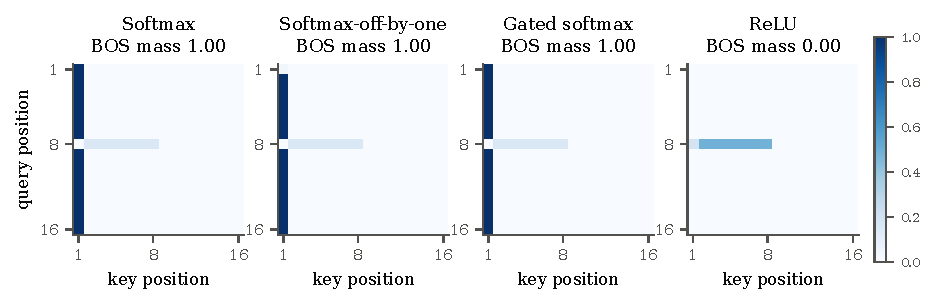
\includegraphics[width=\linewidth]{figures/fig_repro.pdf}
\caption{Mean attention of a trained single-layer, single-head model (trigger at position 8, 1000 test
sequences, seed 0). Softmax, off-by-one and gated attention all park non-trigger rows on \bos{} (column 1);
ReLU switches off instead.}
\label{fig:repro}
\end{figure}

\begin{table}[t]
\caption{Reproduction and variants (5 seeds each). ``Max BOS'': largest per-head \bos{} mass on non-trigger rows,
mean $\pm$ std over seeds. ``Sink heads'': heads with \bos{} mass $>0.6$, summed over seeds. $D$L$H$H: $D$ layers, $H$ heads.}
\label{tab:main}
\centering
\small
\setlength{\tabcolsep}{4.5pt}
\begin{tabular}{llccccc}
\toprule
Model & Attention & Conv. & Steps & Max BOS & Sink heads & Gate off / trig. \\
\midrule
\multirow{6}{*}{1L1H} & softmax & 5/5 & 905 & $1.00\pm.00$ & 5/5 & -- \\
 & off-by-one & 5/5 & 911 & $1.00\pm.00$ & 5/5 & -- \\
 & gated & 5/5 & 1002 & $1.00\pm.00$ & 5/5 & 0.51 / 0.79 \\
 & ReLU & 5/5 & 692 & $0.00\pm.00$ & 0/5 & -- \\
 & sigmoid & 0/5 & -- & -- & -- & -- \\
 & sigmoid-n & 5/5 & 831 & $0.18\pm.03$ & 0/5 & -- \\
\midrule
\multirow{4}{*}{2L2H} & softmax & 5/5 & 10509 & $1.00\pm.00$ & 20/20 & -- \\
 & off-by-one & 5/5 & 8921 & $1.00\pm.00$ & 20/20 & -- \\
 & gated & 5/5 & 9794 & $1.00\pm.00$ & 20/20 & 0.45 / 0.66 \\
 & ReLU / sigmoid-n & 5/5 & -- & $0.00$ / $0.13$ & 0/20 & -- \\
\midrule
\multirow{4}{*}{4L4H} & softmax & 5/5 & 22379 & $1.00\pm.00$ & 37/80 & -- \\
 & off-by-one & 5/5 & 18155 & $0.89\pm.10$ & 40/80 & -- \\
 & gated & 5/5 & 16816 & $0.99\pm.01$ & 38/80 & 0.47 / 0.59 \\
 & ReLU / sigmoid-n & 5/5 & -- & $0.00$ / $0.16$ & 0/80 & -- \\
\bottomrule
\end{tabular}
\end{table}

\section{A sink is not necessary when the head can switch off}
\label{sec:constructions}
The proofs of \citet{ranmilo2026sinks} rely on the head's output being a normalised average of values.
Gating multiplies that average by a query-dependent factor, and off-by-one lets the weights sum to less than
one, so neither is covered. We show both admit sink-free solutions, in the spirit of the paper's ReLU
construction (Thm.~3). Let $W_K=W_V=W_O=I$ and write the score as $s_{ik}=x_i^\top B\,x_k$.

\begin{proposition}[Gated attention]
\label{prop:gated}
Let $B=-c\,(e_\text{trig}+e_\text{cont})e_\text{bos}^\top$ and $g_i=\sigma\!\big(a\,(x_i[\text{trig}]-x_i[\text{cont}]-x_i[\text{bos}])\big)\mathbf{1}$.
Then every non-\bos{} query gives score $-c$ to \bos{} and $0$ to all other keys, so
$\alpha_{i,\bos}=e^{-c}/(e^{-c}+i)\le e^{-c}$ at \emph{every} row. The gate equals $\sigma(a)$ at the trigger and
$\sigma(-a)$ elsewhere. Since inputs are bounded, the maximum error over all inputs is $O(e^{-a}+e^{-c})$.
Hence for any $\varepsilon>0$ there are weights with loss $\le\varepsilon$ and \bos{} mass $\le\varepsilon$ at all
non-trigger rows.
\end{proposition}

\begin{proposition}[Softmax-off-by-one]
\label{prop:off}
Let $B=m\big[e_\text{trig}(e_\text{trig}+e_\text{cont}-e_\text{bos})^\top-(e_\text{bos}+e_\text{cont})(e_\text{bos}+e_\text{trig}+e_\text{cont})^\top\big]$.
The trigger query scores $+m$ on every non-\bos{} key and $-m$ on \bos{}, so its weights tend to the uniform
average over positions $1..j$. Every other query scores $-m$ on all keys, so its total mass is
$\le i\,e^{-m}$ and it outputs $\approx0$ through the null slot. Again the error is $O(L e^{-m})$ and the
\bos{} mass vanishes.
\end{proposition}

\Cref{tab:constr} evaluates both constructions numerically on 2000 random sequences. Already at scale 10,
both reach an error far below the training threshold with essentially zero \bos{} attention. Notably, the
gated solution uses a \emph{query-independent} attention pattern and puts all of the conditional behaviour
into the gate.

\begin{table}[t]
\caption{Explicit sink-free solutions (\cref{prop:gated,prop:off}) evaluated on 2000 sequences.
The training stopping threshold is $\ell_\infty<5\times10^{-3}$.}
\label{tab:constr}
\centering
\small
\begin{tabular}{rcccccccc}
\toprule
 & \multicolumn{3}{c}{Gated} & & \multicolumn{4}{c}{Softmax-off-by-one} \\
\cmidrule{2-4}\cmidrule{6-9}
Scale & MSE & $\ell_\infty$ & BOS mass & & MSE & $\ell_\infty$ & BOS mass & Row mass \\
\midrule
2  & $1.5\!\times\!10^{-3}$ & 0.174 & $2.9\!\times\!10^{-2}$ & & $1.8\!\times\!10^{-2}$ & 0.625 & $6.6\!\times\!10^{-2}$ & 0.51 \\
5  & $5.2\!\times\!10^{-6}$ & 0.010 & $1.5\!\times\!10^{-3}$ & & $2.3\!\times\!10^{-4}$ & 0.086 & $6.4\!\times\!10^{-3}$ & 0.056 \\
10 & $2.4\!\times\!10^{-10}$ & $10^{-4}$ & $1.0\!\times\!10^{-5}$ & & $1.2\!\times\!10^{-8}$ & $6\!\times\!10^{-4}$ & $4.5\!\times\!10^{-5}$ & $4\!\times\!10^{-4}$ \\
20 & $\approx0$ & $\approx0$ & $4.6\!\times\!10^{-10}$ & & $\approx0$ & $\approx0$ & $2.1\!\times\!10^{-9}$ & $2\!\times\!10^{-8}$ \\
\bottomrule
\end{tabular}
\end{table}

\section{\dots{} but training learns the sink anyway}
\label{sec:learned}
\textbf{Gated attention sinks like softmax.} Despite \cref{prop:gated}, every trained gated model in
\cref{tab:main} parks non-trigger rows on \bos{}, with as many sink heads as softmax (38/80 vs.\ 37/80 at
4 layers). The gate barely moves from its initial value of $0.5$: it ends at about $0.45$--$0.5$ on
non-trigger rows and $0.6$--$0.8$ on the trigger row. This is a mild modulation, not a switch. The sink
does the switching.

\textbf{Gate initialisation does not help.} One might expect a gate that starts nearly closed to be used as a
switch. It is not (\cref{fig:gateinit} in \cref{app:more}). With the gate initialised at $\sigma(-4)=0.02$
or $\sigma(-2)=0.12$, \emph{all} 80/80 heads become sinks (vs.\ 38/80 at $0.5$). In every setting the
final gate stays close to its initial value (e.g.\ $0.02\to0.02/0.05$ off/trigger).

\textbf{Depth.} \Cref{fig:depth} sweeps depth from 1 to 8 layers with 4 heads per layer. Softmax and gated
attention keep sinks at every depth. A declining fraction of heads are sinks as depth grows, but the
strongest head always has \bos{} mass $\ge0.95$. Off-by-one behaves differently. At 1--2 layers it is
indistinguishable from softmax, but with depth its sinks fade (7/160 sink heads at 8 layers) and mass moves
into the null slot.

\begin{figure}[t]
\centering
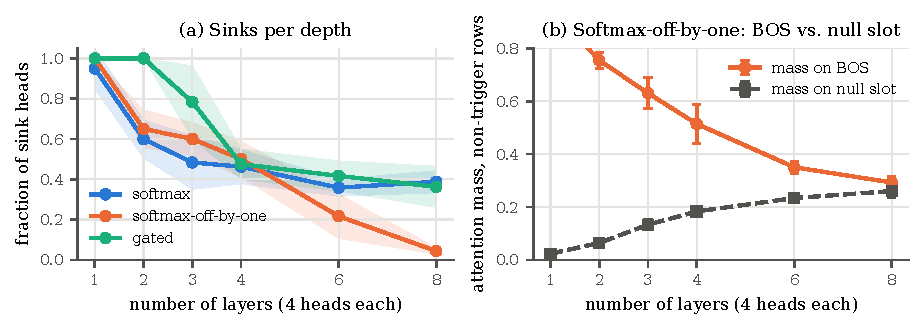
\includegraphics[width=0.92\linewidth]{figures/fig_depth.pdf}
\caption{Depth sweep (4 heads per layer, 5 seeds; band/bars: $\pm1$ std). (a) Fraction of sink heads.
(b) For off-by-one, attention mass on \bos{} vs.\ the null slot, averaged over all heads.}
\label{fig:depth}
\end{figure}

\textbf{Removing the \bos{} token.} If training prefers the sink because a convenient anchor exists, it should
use the off switch once the anchor is gone. We drop \bos{}, so every position is an ordinary content token.
\Cref{tab:nobos} confirms the prediction: off-by-one and gated attention always solve the task, and the gated
model now uses a genuine switch (gate $0.02$ off vs.\ $0.62$ on at one layer). Softmax cannot solve the task
at any depth (0/15 runs) and forms no substitute anchor (no head puts more than $0.21$ on any single key). We
also repeat the experiment with \emph{learned positional embeddings} added to the query and key inputs, which
lets a head single out a position. Softmax still fails and still forms no anchor (maximum $0.20$ on any key,
3 seeds at 1 and 2 layers). The gated model still solves the task with gate $0.01$. This failure is what the
theorem predicts rather than a counter-example to it: an anchor is only useful if its value is constant, and
without \bos{} every token's value carries random content. The expectation of \citet[Sec.~5]{ranmilo2026sinks}
that a suppressed sink ``reappears elsewhere'' therefore needs a token with a constant value, such as a
delimiter or a repeated special token, to be tested.

\begin{table}[t]
\caption{Training without a \bos{} token (5 seeds per cell). ``Mass'': mean total attention
$\sum_k\alpha_{ik}$ on non-trigger rows (1 for softmax and gated by construction).}
\label{tab:nobos}
\centering
\small
\begin{tabular}{lccc}
\toprule
Attention & 1 layer, 1 head & 2 layers, 2 heads & 4 layers, 4 heads \\
\midrule
softmax & 0/5 ($\ell_\infty=0.74$) & 0/5 ($0.70$) & 0/5 ($0.08$) \\
off-by-one & 5/5, mass $0.00$ & 5/5, mass $0.42$ & 5/5, mass $0.57$ \\
gated & 5/5, gate $0.02$ / $0.62$ & 5/5, gate $0.28$ / $0.63$ & 5/5, gate $0.41$ / $0.64$ \\
ReLU, sigmoid-n & 5/5 & 5/5 & 5/5 \\
\bottomrule
\end{tabular}
\end{table}

\section{Why the sink wins: a race between two routes}
\label{sec:race}
On a non-trigger row a gated head can switch off in two ways. It can put its attention on \bos{} (whose value
it can set to zero), or it can close its gate. We call these the sink route and the gate route.

\textbf{Gradient probes.} We add two zero-valued probe scalars per head, active only on non-trigger rows:
$p_\text{sink}$ is added to the \bos{} attention logit and $p_\text{gate}$ to the gate pre-activation. They
leave the forward pass unchanged, and their gradients show which route the loss pulls on. \Cref{fig:probe}(a)
corrects an earlier version of this analysis. Because $p_\text{gate}$ acts on all $d_h=16$ gate coordinates
at once, its raw gradient is a \emph{sum} over 16 coordinates and looks larger than the sink pull (peak
$6.2\times10^{-4}$ vs.\ $3.9\times10^{-4}$). Per coordinate, the gate pull is only $0.1$--$0.4\times$ the
sink pull. Under Adam the size of a gradient does not set the size of an update in any case. The question is
therefore which route \emph{moves} faster, not which one the loss prefers.

\textbf{Trajectories.} \Cref{fig:probe}(b,c) tracks the \bos{} logit gap $s$ (the \bos{} logit minus the mean
logit of the other keys) and the gate closing $-z$ (minus the mean gate pre-activation) on non-trigger rows.
At $\lambda=1$ the sink logit rises quadratically, $s\approx at^2$, while the gate barely moves; the run ends
with $s\approx11.5$, $-z\approx0$. At $\lambda=10$ the gate closes linearly, $-z\approx bt$, and gets an early
lead. The quadratic sink then catches up, and both routes end with a share of the work ($s\approx7$,
$-z\approx5$, \bos{} mass $0.99$, gate $0.01$).

\begin{figure}[t]
\centering
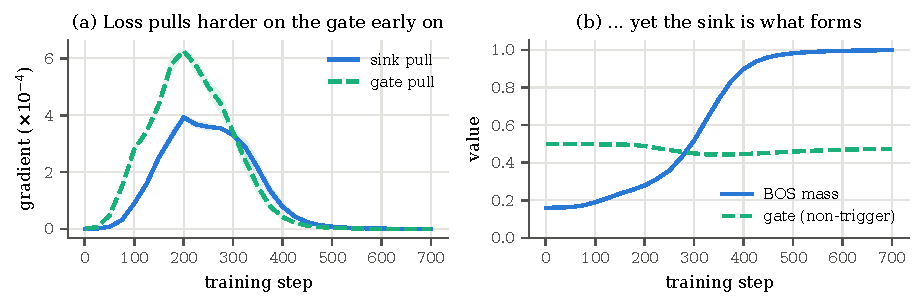
\includegraphics[width=\linewidth]{figures/fig_probe.pdf}
\caption{Single-layer gated model, 3 seeds. (a) Probe gradients: the gate pull is large only when summed
over its 16 coordinates (dotted); per coordinate it is far smaller than the sink pull. (b, c) The two routes'
logits on non-trigger rows: the sink grows like $t^2$, the gate like $t$ (dotted: early-phase fits).}
\label{fig:probe}
\end{figure}

\textbf{Controls.} \Cref{tab:controls} intervenes on the speed of each route in the 4-layer model. A $10\times$
gate learning rate removes every sink (0/48 heads). Speeding up \emph{also} the query and key weights
($W_Q,W_K$, the factors of the sink logit) by $10\times$ turns every head into a sink (48/48). Raising
\emph{all} learning rates by $10\times$ trains just as fast but keeps 33/48 sinks. So the effect is the
relative speed of the two routes, not the amount of learning rate. It also shows that the speed-up in
training time is a property of a larger learning rate rather than of the gate. A single scalar gate per head
behaves like the elementwise gate.

\begin{table}[t]
\caption{Controls (4 layers $\times$ 4 heads, $d_h=16$, 3 seeds, all converged). Gate values are
importance-weighted, on non-trigger / trigger rows.}
\label{tab:controls}
\centering
\small
\begin{tabular}{lcccc}
\toprule
Configuration & Sink heads & Mean BOS & Gate off / trig. & Steps \\
\midrule
baseline ($\lambda=1$) & 23/48 & 0.57 & 0.47 / 0.58 & 18.4k \\
gate lr $\times10$ ($\lambda=10$) & \textbf{0/48} & 0.20 & 0.16 / 0.71 & 3.3k \\
gate lr $\times10$ and $W_Q,W_K$ lr $\times10$ & \textbf{48/48} & 1.00 & 0.74 / 0.91 & 3.4k \\
all lr $\times10$ & 33/48 & 0.74 & 0.43 / 0.58 & 3.4k \\
scalar gate per head, $\lambda=1$ & 28/48 & 0.63 & 0.44 / 0.60 & 12.8k \\
scalar gate per head, $\lambda=10$ & 0/48 & 0.32 & 0.04 / 0.74 & 4.2k \\
\bottomrule
\end{tabular}
\end{table}

\section{A quantitative theory of the race}
\label{sec:theory}
\textbf{Minimal model.} Consider one non-trigger row of a gated head. Ignoring the other heads, its output is
$g_i\odot(1-\alpha_{i,\bos})\bar v_i$, where $\bar v_i$ is the attention-weighted mean of the non-\bos{} values.
With $i$ non-\bos{} keys, $1-\alpha_{i,\bos}\approx i\,e^{-s}$ and $\sigma(z)\approx e^{z}$ when the routes
are well under way. The row's error is therefore
\begin{equation}
\log \text{err} \;\approx\; \log(C\,i) \;-\; s \;-\; (-z), \qquad C=\|\bar v\|_\infty .
\label{eq:budget}
\end{equation}
Training stops when $\text{err}<\varepsilon$, so at that moment
\begin{equation}
s^* + (-z^*) \;\approx\; T' := \log(C\,i/\varepsilon).
\label{eq:share}
\end{equation}
The two routes \emph{share one budget}. Whatever the sink has done when training stops, the gate does not
have to do, and the other way round.

\textbf{Speeds under Adam.} With a small learning rate $\eta$, Adam moves each weight by about $\eta$ per step as
long as the sign of its gradient is stable. The sink logit is a sum of $d_h$ products,
$s=\sum_{r\le d_h}W_Q[r,\text{cont}]\,W_K[r,\text{bos}]$. Each factor grows linearly, so
$s(t)\approx d_h(\eta t)^2$. The gate logit $z=W_G[\cdot,\text{cont}]+b_G$ is linear in two weights whose
learning rate is $\lambda\eta$, so $-z(t)\approx 2\lambda\eta t$. Writing $u=\eta t$, training stops at
$d_hu^2+2\lambda u=T'$. The head ends as a sink ($\alpha_\bos>a_0=0.6$) iff
$s^*=d_hu^{*2}>S_0:=\log(i\,a_0/(1-a_0))$. Solving for the multiplier at which this switches,
\begin{equation}
\lambda^*(d_h) \;=\; \frac{T'-S_0}{2\sqrt{S_0}}\,\sqrt{d_h}.
\label{eq:lamstar}
\end{equation}
This gives three testable predictions.
\textbf{(P1)} the routes share a constant budget, \cref{eq:share};
\textbf{(P2)} $\eta$ cancels, so the outcome does not depend on the base learning rate;
\textbf{(P3)} $\lambda^*$ grows like $\sqrt{d_h}$.
With $i=8$, $\varepsilon=5\times10^{-3}$ and $C=1$ we get $T'=7.4$, $S_0=2.5$ and $\lambda^*\approx1.55\sqrt{d_h}$.
A direct simulation of the minimal model with real Adam (not the sign approximation; \texttt{race\_theory.py})
agrees with the closed form (\cref{fig:race}a). Under SGD the analysis changes: the sink's gradient is
proportional to the other factor, which starts at $O(0.02)$. The minimal model therefore predicts
\textbf{(P4)}: with SGD the gate always wins.

\textbf{Tests.} We sweep $d_h\in\{4,\dots,64\}$ and $\lambda\in\{1,\dots,128\}$ in the 1-layer, 4-head residual
model (3 seeds per cell; \cref{fig:race}b,c).
\begin{itemize}
  \item \textbf{P1 holds.} Across all 1-layer runs, $s^*+(-z^*)=8.8\pm1.8$ per head, and the two are strongly
        anti-correlated ($r=-0.83$; \cref{fig:lr}b). The budget is larger than our rough constant
        ($T'\approx7.4$) because the true $C$ and $i$ differ from the values we assumed.
  \item \textbf{P2 holds.} At base learning rates $3\times10^{-5}$, $10^{-4}$ and $3\times10^{-4}$ the \bos{} mass
        vs.\ $\lambda$ curves are indistinguishable (\cref{fig:lr}a). Training takes $10\times$ more steps at
        the smallest rate, but the outcome is the same.
  \item \textbf{P3 holds up to a constant.} $\lambda^*$ is $14.5$, $21.8$, $29.9$ and $46.0$ at $d_h=4,8,16,32$.
        The fitted log-log slope is $0.55$ (theory $0.5$), and every value is $4.8\pm0.2\times$ the closed form.
        The exception is $d_h=64$ ($\lambda^*=24$), where the head is wider than the model ($d=16$): $W_OW_V$ has
        rank at most 16, so only a quarter of the gate coordinates matter. The gate route is slower than the two-weight idealisation
        assumes, because its gradient sign is noisy: it is driven by random content and opposed on the trigger row.
  \item \textbf{P4 fails.} With SGD (momentum 0.9, lr 30; 3 seeds), gated models still form sinks in 5 of 12 heads.
        In the full model the gate's gradient is itself proportional to the small value and output weights, a
        coupling the minimal model leaves out. So both routes start slowly under SGD.
\end{itemize}
In deeper models the race is less width-dependent: at 4 layers, $\lambda=10$ is enough at every width tested
(\cref{sec:fix}). This is plausibly because several heads can cancel each other's leftover output, which
gives the network a third way to switch off.

\begin{figure}[t]
\centering
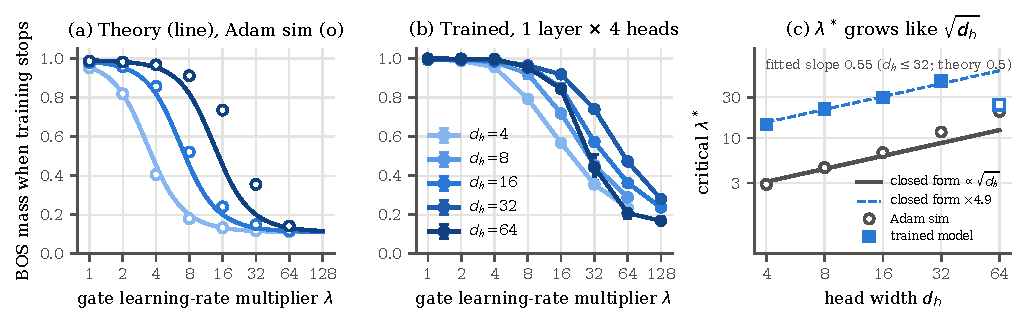
\includegraphics[width=\linewidth]{figures/fig_race.pdf}
\caption{The critical gate multiplier. (a) Minimal model: closed form (lines) and Adam simulation (circles).
(b) Trained 1-layer, 4-head models (3 seeds): \bos{} mass vs.\ $\lambda$ per head width; dashed: sink
threshold. (c) $\lambda^*$ (where the \bos{} mass crosses 0.6) vs.\ $d_h$.}
\label{fig:race}
\end{figure}

\begin{figure}[t]
\centering
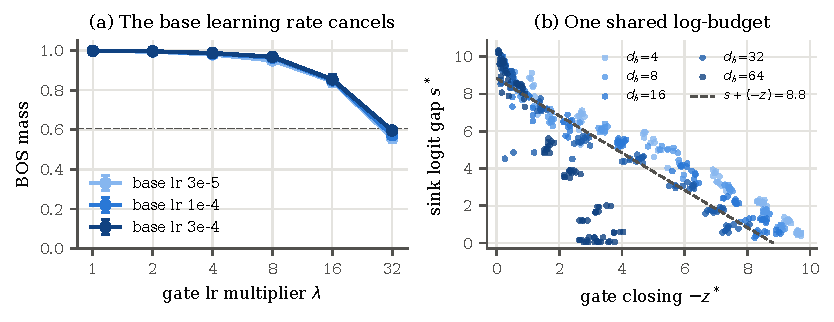
\includegraphics[width=0.8\linewidth]{figures/fig_lr.pdf}
\caption{(a) $d_h=16$: changing the base learning rate $10\times$ does not change the race (3 seeds per point).
(b) One point per head of every 1-layer run: sink logit gap vs.\ gate closing at the stopping point. They
trade off along $s+(-z)=$const, as predicted by \cref{eq:share}.}
\label{fig:lr}
\end{figure}

\section{Changing the race: gate parameterisations}
\label{sec:fix}
If the outcome is a race, the gate can be made to win by changing its parameterisation instead of
hand-tuning a learning rate. We compare four gates in the 4-layer model at $d_h\in\{4,16,64\}$ and depth
1, 4 and 8 (\cref{fig:fix}, 3 seeds each):
\begin{itemize}
  \item the \textbf{linear gate} of \citet{qiu2025gated} at $\lambda=1$ and $\lambda=10$;
  \item a \textbf{race-matched gate} $g=\sigma(\kappa(W_Gx+b))$ with $\kappa=2.5\sqrt{d_h}$ and $W_G$ initialised
        at $0.02/\kappa$. It computes the same function as the linear gate at initialisation and under Adam is
        exactly $\lambda=\kappa$. The constant 2.5 matches the validated $\lambda=10$ at $d_h=16$, and the $\sqrt{d_h}$
        rule comes from \cref{eq:lamstar};
  \item a \textbf{bilinear gate} $z=A_h(B_hx)+b$, a product of two learned factors like the sink. The theory
        predicts that a symmetric race splits the budget evenly, giving partial sinks independent of $d_h$.
\end{itemize}
\textbf{Results.}
\begin{itemize}
  \item The race-matched gate is sink-free at $d_h=16$ and $64$ (0/48 each) and at 8 layers (0/96). It is also
        the fastest to converge (1.7k steps at $d_h=64$ vs.\ 9.8k at $\lambda=1$).
  \item At $d_h=4$ it fails (23/48 sinks with $\kappa=5$), while the fixed $\lambda=10$ succeeds at all three
        widths. In the 4-layer model the $\sqrt{d_h}$ rule therefore scales the gate down too much for narrow
        heads.
  \item The bilinear gate gives partial sinks, as predicted (mean \bos{} $0.32$--$0.66$). It is not a fix.
\end{itemize}
The practical recommendation is a gate learning-rate multiplier of order 10 at 4--8 layers. At one layer,
$\lambda^*$ grows with width and a larger multiplier is needed (\cref{fig:race}c). \Cref{tab:glr} in
\cref{app:more} lists the full $\lambda$ sweep.

\begin{figure}[t]
\centering
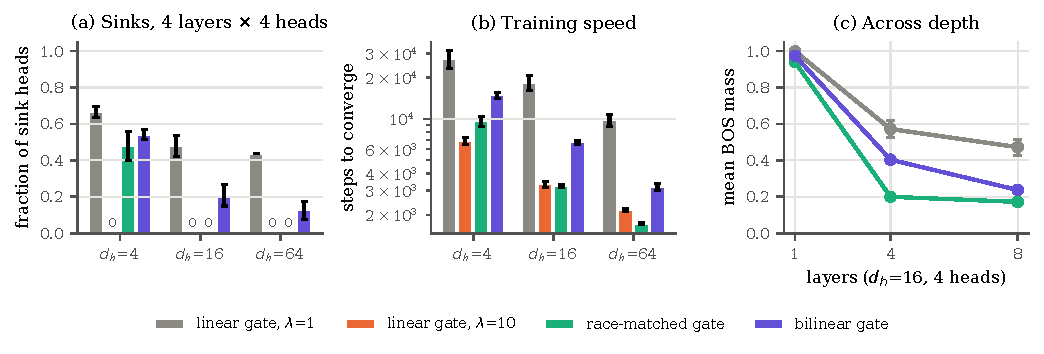
\includegraphics[width=\linewidth]{figures/fig_fix.pdf}
\caption{Gate parameterisations (3 seeds). (a) Fraction of sink heads at 4 layers $\times$ 4 heads, by head
width. (b) Steps to converge. (c) Mean \bos{} mass vs.\ depth at $d_h=16$.}
\label{fig:fix}
\end{figure}

\section{A small language model}
\label{sec:lm}
Does the race carry over to a real language model? We train character-level GPTs on TinyStories
(\texttt{lm.py}): 6 layers, $d=384$, 6 heads of width 64, pre-LayerNorm with MLPs, learned positional
embeddings, context 256, AdamW ($\beta=(0.9,0.95)$, weight decay 0.1, cosine schedule), batch 64, mixed
precision on Kaggle T4s, about 11M parameters. Every sequence starts with a \bos{} token. We compare softmax,
off-by-one, the linear gate at $\lambda=1$ and $\lambda=10$, and the race-matched gate ($\kappa=2.5\sqrt{64}=20$).

\textbf{Run 1} (first 255 characters of each story, 8k steps, learning rate $10^{-3}$, 2 seeds;
\cref{fig:lm}). After 131M characters \emph{no} variant has an attention sink. Mean attention on \bos{} is
0.02 for all of them, the uniform level, and the strongest \bos{} head reaches only 0.15. This agrees with
\citet{gu2025when}, who find that sinks emerge only after sufficient training. What we do see is the
\emph{precursor} of a sink, a massive activation at the \bos{} position. In softmax models the largest
hidden-state entry at \bos{} is $1.43\times$ the largest anywhere else (layers 2--5), and off-by-one is close
($1.39\times$). Gating weakens this outlier in the order the race predicts: $1.22\times$ at $\lambda=1$, and
none at all at $\lambda=10$ ($0.97\times$) or with the race-matched gate ($1.01\times$). The strongest \bos{} head
follows the same order (0.15, 0.14, 0.13, 0.08, 0.07). Faster gates cost a little language-modelling loss
(0.390 for softmax and $\lambda=1$ vs.\ 0.393 and 0.397 nats/char) at this short training length.

\textbf{Run 2} (packed chunks from random offsets, as in standard pre-training; 20k steps, learning rate
$2\times10^{-3}$, 1 seed; \cref{fig:lm2} in \cref{app:more}) was designed to make sinks form, but still has
none: the strongest \bos{} head reaches 0.33 (softmax), 0.27 (gate, $\lambda=10$), 0.18 ($\lambda=1$) and 0.11
(off-by-one). The \bos{} activation outlier is now similar in all variants ($1.26$--$1.33\times$), so the
ordering seen in run 1 does not hold under packed training. Many heads in every variant put almost all of their
attention on a single key (up to 0.99), but we did not record which key, and in a character-level model such
heads may simply be previous-character heads. Gating slightly \emph{improves} the loss here (0.506 at
$\lambda=1$ vs.\ 0.520 for softmax, one seed), in line with \citet{qiu2025gated}. Overall, at this scale and
training length the language model does not test the race. Whether a fast gate removes sinks once they form in
real language models remains open.

\begin{figure}[t]
\centering
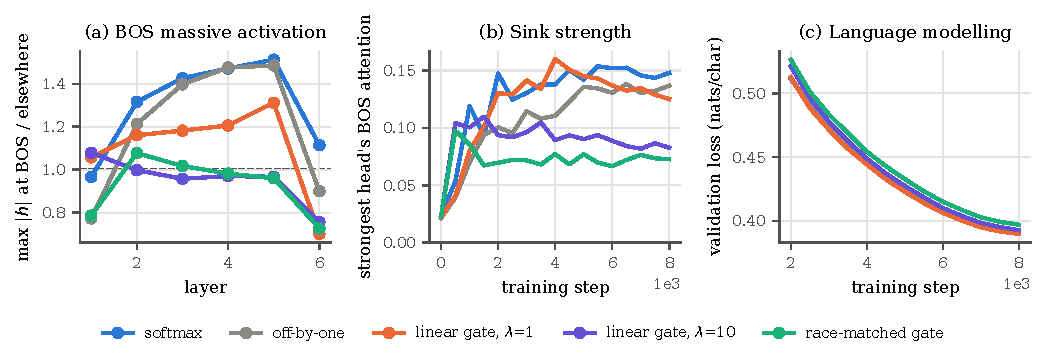
\includegraphics[width=\linewidth]{figures/fig_lm.pdf}
\caption{Character-level GPT on TinyStories, run 1 (2 seeds, 8k steps). (a) Largest hidden-state entry at
\bos{} divided by the largest elsewhere, per layer, at the end of training: softmax and off-by-one build a
\bos{} outlier, fast gates do not. (b) Attention of the most \bos{}-focused head during training. (c)
Validation loss.}
\label{fig:lm}
\end{figure}

\section{Discussion}
\textbf{Implications for the original paper.} \citet{ranmilo2026sinks} show what softmax \emph{needs}; we
show what training \emph{prefers}. Adding an off switch makes the sink unnecessary, but it does not by itself
make a model sink-free, because gradient descent can reach the sink first. Whether it does is decided by a race
whose structure we can predict: a shared log-budget and invariance to the base learning rate. Its threshold
depends on head width and depth.

\textbf{Relation to gated LLMs.} \citet{qiu2025gated} observe far fewer sinks with gating at scale, while
\citet{rizwan2026new} do not at small scale. The race offers a common explanation. Whether the gate wins
depends on the relative speed of the two routes, which depends on head width, depth, normalisation layers,
initialisation, the per-parameter learning rate and training length, and all of these differ between the two
studies. Our results suggest checking gate statistics early in training and raising the gate's learning
rate when sink-free behaviour is desired.

\textbf{Limitations.}
\begin{itemize}
  \item Most experiments use the synthetic task and attention-only models of the original paper: no MLPs,
        LayerNorm or positional encoding, sequence length 16 and width 16.
  \item The constructions are existence results, not a characterisation of all solutions.
  \item The race theory is a first-order sign-Adam argument. It predicts the budget and the learning-rate
        invariance well, but it gets the size of $\lambda^*$ wrong by a factor of 4--5 and fails for SGD.
  \item The language models are small and no sink formed in them within 20k steps (\cref{sec:lm}), so the
        race is established on the synthetic task only.
  \item Some numbers differ slightly between CPU and GPU runs of the same seed. All the controls in
        \cref{tab:controls,tab:glr} are compared within one device.
\end{itemize}

\section{Conclusion}
Attention sinks are necessary for softmax, and they are also \emph{preferred} by training whenever a stable
anchor exists, even in architectures that could do without them. In a controlled setting we showed that gated
and off-by-one attention admit sink-free solutions, yet gradient descent reliably builds sinks in them because
the bilinear sink outruns the linear gate. We turned this into a quantitative race with a conserved
log-budget and a learning-rate-invariant threshold, confirmed its main predictions, and identified where it
breaks down. Removing the anchor, adding depth, or giving the gate a large enough learning-rate multiplier
shifts the race towards the gate.

\paragraph{Code.} All code, configurations and raw results are included with this submission
(\url{https://github.com/Adityakariwal/fllm-final-project}). Every number and figure can be regenerated with \texttt{reproduce.sh}, and
\texttt{src/summarize.py} recomputes every table entry from the raw results.

\bibliography{references}
\bibliographystyle{iclr2025_conference}

\appendix
\section{Implementation details}
\label{app:impl}
\textbf{Code.} We re-implemented the task and models from scratch in PyTorch, following the released
reference code of \citet{ranmilo2026sinks} for data generation, initialisation, optimiser and stopping
rule. Differences from the reference: batched data generation on the device, additional attention variants,
head width $d_h$, gate parameterisations, probes and tracking. The reference stopping threshold
($5\times10^{-3}$, from the code) is used throughout.

\textbf{Hyper-parameters.} $d=16$, $L=16$, batch 128, Adam $(0.9,0.95)$, no weight decay, initialisation
$\mathcal{N}(0,0.02^2)$ for all weights, gate bias $0$ unless stated. Learning rate $10^{-3}$ for
single-layer non-residual models (\cref{tab:main} top block, gate-LR 1-layer sweep, probes) and $10^{-4}$
otherwise. The depth sweep and the race sweeps of \cref{sec:theory} use residual models with 4 heads for all
depths, including $D=1$. Maximum steps: 50k (80k for 6 and 8 layers); the no-\bos{} 1-layer sweep was capped
at 20k steps. SGD runs use momentum 0.9 and learning rate 30. This is the only rate in $\{1,10,30\}$ that
converges within 6k steps; the loss is a mean over $128\times16\times16$ entries, so gradients are small.

\textbf{No-\bos{} variant.} Position $0$ becomes a content token, the trigger is sampled from
$\{1,\dots,15\}$, and the target averages positions $0..j$. ReLU and sigmoid-n divide by the number of
non-\bos{} keys, which is $i+1$ without \bos{} instead of $i$. The positional-embedding variant adds a learned
$\mathcal{N}(0,0.02^2)$ embedding to the query and key inputs only, so the target is unchanged.

\textbf{Probes.} Every 25 steps we draw 512 fresh sequences, add zero scalars $p_\text{sink}$ (to the
\bos{} logit) and $p_\text{gate}$ (to the gate pre-activation, all coordinates) on non-trigger rows of each
head, and record $-\partial L/\partial p_\text{sink}$ and $\partial L/\partial p_\text{gate}$ (the latter both
summed over and divided by the $d_h$ coordinates). Probes are removed before the optimisation step, so
training is unaffected.

\textbf{Compute.} Single-layer and shallow sweeps ran on a laptop CPU. Deeper sweeps of the original study
ran on Kaggle ($2\times$ NVIDIA T4). The race sweeps of \cref{sec:race,sec:theory,sec:fix} ran on 11 CPU
cores, and the language models on Kaggle T4s. In total we trained 558 models (312 in the original study,
232 in the race sweeps, 14 language models), plus 6 probe runs.

\section{Additional results}
\label{app:more}
\begin{figure}[h]
\centering
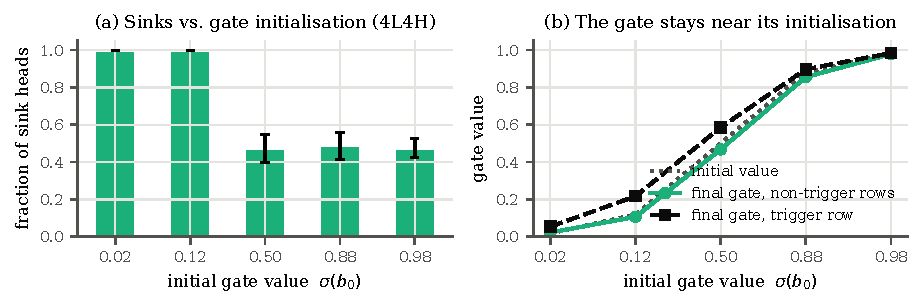
\includegraphics[width=0.85\linewidth]{figures/fig_gateinit.pdf}
\caption{Gated attention, 4 layers $\times$ 4 heads, 5 seeds per bar. (a) A nearly closed initial gate turns
every head into a sink. (b) The trained gate stays near its initialisation (dotted) instead of becoming an
on/off switch.}
\label{fig:gateinit}
\end{figure}

\begin{figure}[h]
\centering
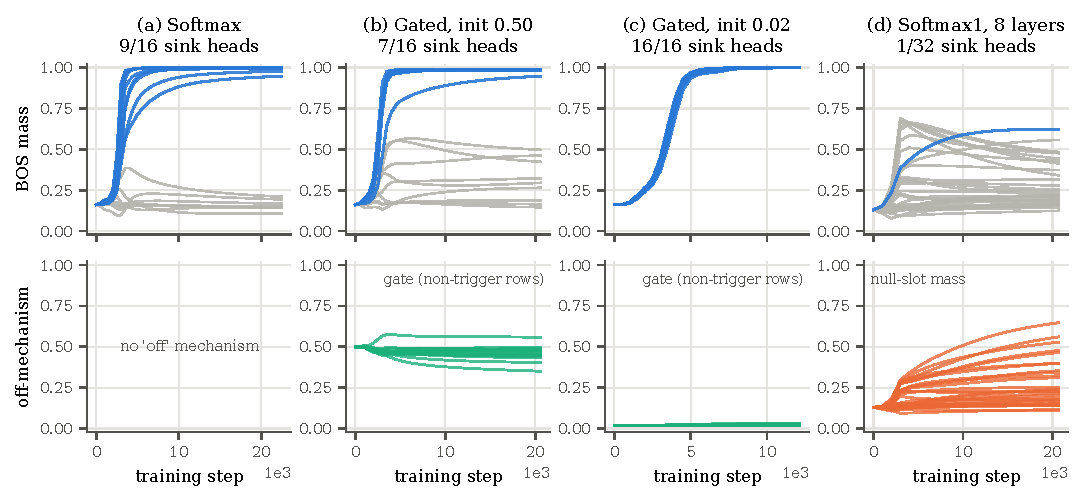
\includegraphics[width=\linewidth]{figures/fig_timelines.pdf}
\caption{Training timelines (seed 0, 4 layers $\times$ 4 heads unless noted). Top: \bos{} mass per head
(blue: heads that end as sinks). Bottom: the head's off mechanism, i.e.\ gate value (green) or null-slot
mass (orange). Sinks appear abruptly (an S-shaped rise between roughly 2k and 5k steps) and never reverse in
softmax and gated models. In deep off-by-one models sinks form first and are then slowly replaced by
null-slot mass.}
\label{fig:timelines}
\end{figure}

\begin{figure}[h]
\centering
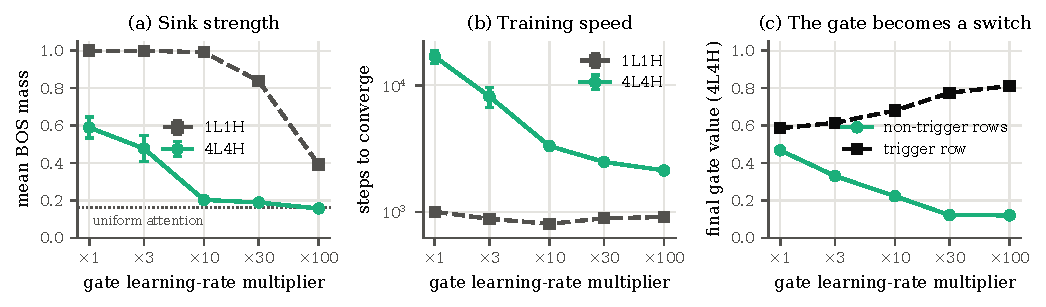
\includegraphics[width=\linewidth]{figures/fig_gatelr.pdf}
\caption{Gate learning-rate multiplier in the original configurations (5 seeds per point). (a) Sink strength.
(b) Steps to converge. (c) Final gate values at 4 layers (mean over coordinates).}
\label{fig:gatelr}
\end{figure}

\begin{table}[h]
\caption{Gate learning-rate multiplier $\lambda$ in the original configurations (gated attention, 5 seeds
each, all converged). At 1 layer, $\lambda=10$ closes the gate \emph{and} keeps the sink: the two routes share
the budget (\cref{sec:theory}). At 4 layers the mean gate stays at $0.12$--$0.33$ on non-trigger rows. Even
there the no-op is not achieved by the gate alone; partial gating combines with heads cancelling each other.}
\label{tab:glr}
\centering
\small
\begin{tabular}{rcccccc}
\toprule
 & \multicolumn{3}{c}{1 layer, 1 head} & \multicolumn{3}{c}{4 layers, 4 heads} \\
\cmidrule(lr){2-4}\cmidrule(lr){5-7}
$\lambda$ & BOS mass & Gate off/trig. & Steps & Sink heads & Gate off/trig. & Steps \\
\midrule
1   & 1.00 & 0.50 / 0.78 & 1004 & 38/80 & 0.47 / 0.59 & 16816 \\
3   & 1.00 & 0.33 / 0.93 & 885  & 25/80 & 0.33 / 0.61 & 8161 \\
10  & 0.99 & 0.01 / 0.99 & 807  & 0/80  & 0.22 / 0.68 & 3315 \\
30  & 0.84 & 0.00 / 1.00 & 894  & 0/80  & 0.12 / 0.77 & 2484 \\
100 & 0.39 & 0.00 / 1.00 & 915  & 0/80  & 0.12 / 0.81 & 2130 \\
\bottomrule
\end{tabular}
\end{table}

\begin{figure}[h]
\centering
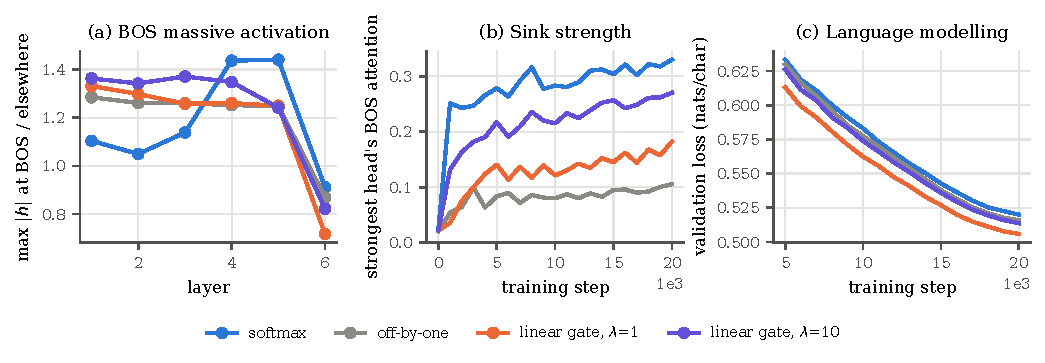
\includegraphics[width=\linewidth]{figures/fig_lm2.pdf}
\caption{Language model, run 2 (packed random-offset chunks, 20k steps, 1 seed). (a) \bos{} activation outlier
per layer, (b) attention of the most \bos{}-focused head, (c) validation loss. No sink forms, and the variants
no longer differ in the \bos{} outlier.}
\label{fig:lm2}
\end{figure}

\textbf{Sink heads by depth} (5 seeds, 4 heads per layer, sink head: \bos{} mass $>0.6$):
\begin{center}
\small
\begin{tabular}{lcccccc}
\toprule
Layers & 1 & 2 & 3 & 4 & 6 & 8 \\
\midrule
softmax & 19/20 & 24/40 & 29/60 & 37/80 & 43/120 & 62/160 \\
off-by-one & 20/20 & 26/40 & 36/60 & 40/80 & 26/120 & 7/160 \\
\quad null-slot share in sink heads & 0.02 & 0.02 & 0.11 & 0.19 & 0.32 & 0.33 \\
gated & 20/20 & 40/40 & 47/60 & 38/80 & 50/120 & 58/160 \\
\quad gate off / trig. & .42/.66 & .43/.62 & .45/.60 & .47/.59 & .47/.57 & .48/.56 \\
\bottomrule
\end{tabular}
\end{center}

\textbf{Gate initialisation} (4 layers $\times$ 4 heads, 5 seeds): initial gate $0.02$: 80/80 sink heads,
final gate $0.02/0.05$; $0.12$: 80/80, $0.11/0.22$; $0.50$: 38/80, $0.47/0.59$; $0.88$: 39/80,
$0.86/0.90$; $0.98$: 38/80, $0.98/0.98$ (off/trigger).

\end{document}
